\documentclass[1p]{elsarticle_modified}
%\bibliographystyle{elsarticle-num}

%\usepackage[colorlinks]{hyperref}
%\usepackage{abbrmath_seonhwa} %\Abb, \Ascr, \Acal ,\Abf, \Afrak
\usepackage{amsfonts}
\usepackage{amssymb}
\usepackage{amsmath}
\usepackage{amsthm}
\usepackage{scalefnt}
\usepackage{amsbsy}
\usepackage{kotex}
\usepackage{caption}
\usepackage{subfig}
\usepackage{color}
\usepackage{graphicx}
\usepackage{xcolor} %% white, black, red, green, blue, cyan, magenta, yellow
\usepackage{float}
\usepackage{setspace}
\usepackage{hyperref}

\usepackage{tikz}
\usetikzlibrary{arrows}

\usepackage{multirow}
\usepackage{array} % fixed length table
\usepackage{hhline}

%%%%%%%%%%%%%%%%%%%%%
\makeatletter
\renewcommand*\env@matrix[1][\arraystretch]{%
	\edef\arraystretch{#1}%
	\hskip -\arraycolsep
	\let\@ifnextchar\new@ifnextchar
	\array{*\c@MaxMatrixCols c}}
\makeatother %https://tex.stackexchange.com/questions/14071/how-can-i-increase-the-line-spacing-in-a-matrix
%%%%%%%%%%%%%%%

\usepackage[normalem]{ulem}

\newcommand{\msout}[1]{\ifmmode\text{\sout{\ensuremath{#1}}}\else\sout{#1}\fi}
%SOURCE: \msout is \stkout macro in https://tex.stackexchange.com/questions/20609/strikeout-in-math-mode

\newcommand{\cancel}[1]{
	\ifmmode
	{\color{red}\msout{#1}}
	\else
	{\color{red}\sout{#1}}
	\fi
}

\newcommand{\add}[1]{
	{\color{blue}\uwave{#1}}
}

\newcommand{\replace}[2]{
	\ifmmode
	{\color{red}\msout{#1}}{\color{blue}\uwave{#2}}
	\else
	{\color{red}\sout{#1}}{\color{blue}\uwave{#2}}
	\fi
}

\newcommand{\Sol}{\mathcal{S}} %segment
\newcommand{\D}{D} %diagram
\newcommand{\A}{\mathcal{A}} %arc


%%%%%%%%%%%%%%%%%%%%%%%%%%%%%5 test

\def\sl{\operatorname{\textup{SL}}(2,\Cbb)}
\def\psl{\operatorname{\textup{PSL}}(2,\Cbb)}
\def\quan{\mkern 1mu \triangleright \mkern 1mu}

\theoremstyle{definition}
\newtheorem{thm}{Theorem}[section]
\newtheorem{prop}[thm]{Proposition}
\newtheorem{lem}[thm]{Lemma}
\newtheorem{ques}[thm]{Question}
\newtheorem{cor}[thm]{Corollary}
\newtheorem{defn}[thm]{Definition}
\newtheorem{exam}[thm]{Example}
\newtheorem{rmk}[thm]{Remark}
\newtheorem{alg}[thm]{Algorithm}

\newcommand{\I}{\sqrt{-1}}
\begin{document}

%\begin{frontmatter}
%
%\title{Boundary parabolic representations of knots up to 8 crossings}
%
%%% Group authors per affiliation:
%\author{Yunhi Cho} 
%\address{Department of Mathematics, University of Seoul, Seoul, Korea}
%\ead{yhcho@uos.ac.kr}
%
%
%\author{Seonhwa Kim} %\fnref{s_kim}}
%\address{Center for Geometry and Physics, Institute for Basic Science, Pohang, 37673, Korea}
%\ead{ryeona17@ibs.re.kr}
%
%\author{Hyuk Kim}
%\address{Department of Mathematical Sciences, Seoul National University, Seoul 08826, Korea}
%\ead{hyukkim@snu.ac.kr}
%
%\author{Seokbeom Yoon}
%\address{Department of Mathematical Sciences, Seoul National University, Seoul, 08826,  Korea}
%\ead{sbyoon15@snu.ac.kr}
%
%\begin{abstract}
%We find all boundary parabolic representation of knots up to 8 crossings.
%
%\end{abstract}
%\begin{keyword}
%    \MSC[2010] 57M25 
%\end{keyword}
%
%\end{frontmatter}

%\linenumbers
%\tableofcontents
%
\newcommand\colored[1]{\textcolor{white}{\rule[-0.35ex]{0.8em}{1.4ex}}\kern-0.8em\color{red} #1}%
%\newcommand\colored[1]{\textcolor{white}{ #1}\kern-2.17ex	\textcolor{white}{ #1}\kern-1.81ex	\textcolor{white}{ #1}\kern-2.15ex\color{red}#1	}

{\Large $\underline{12n_{0507}~(K12n_{0507})}$}

\setlength{\tabcolsep}{10pt}
\renewcommand{\arraystretch}{1.6}
\vspace{1cm}\begin{tabular}{m{100pt}>{\centering\arraybackslash}m{274pt}}
\multirow{5}{120pt}{
	\centering
	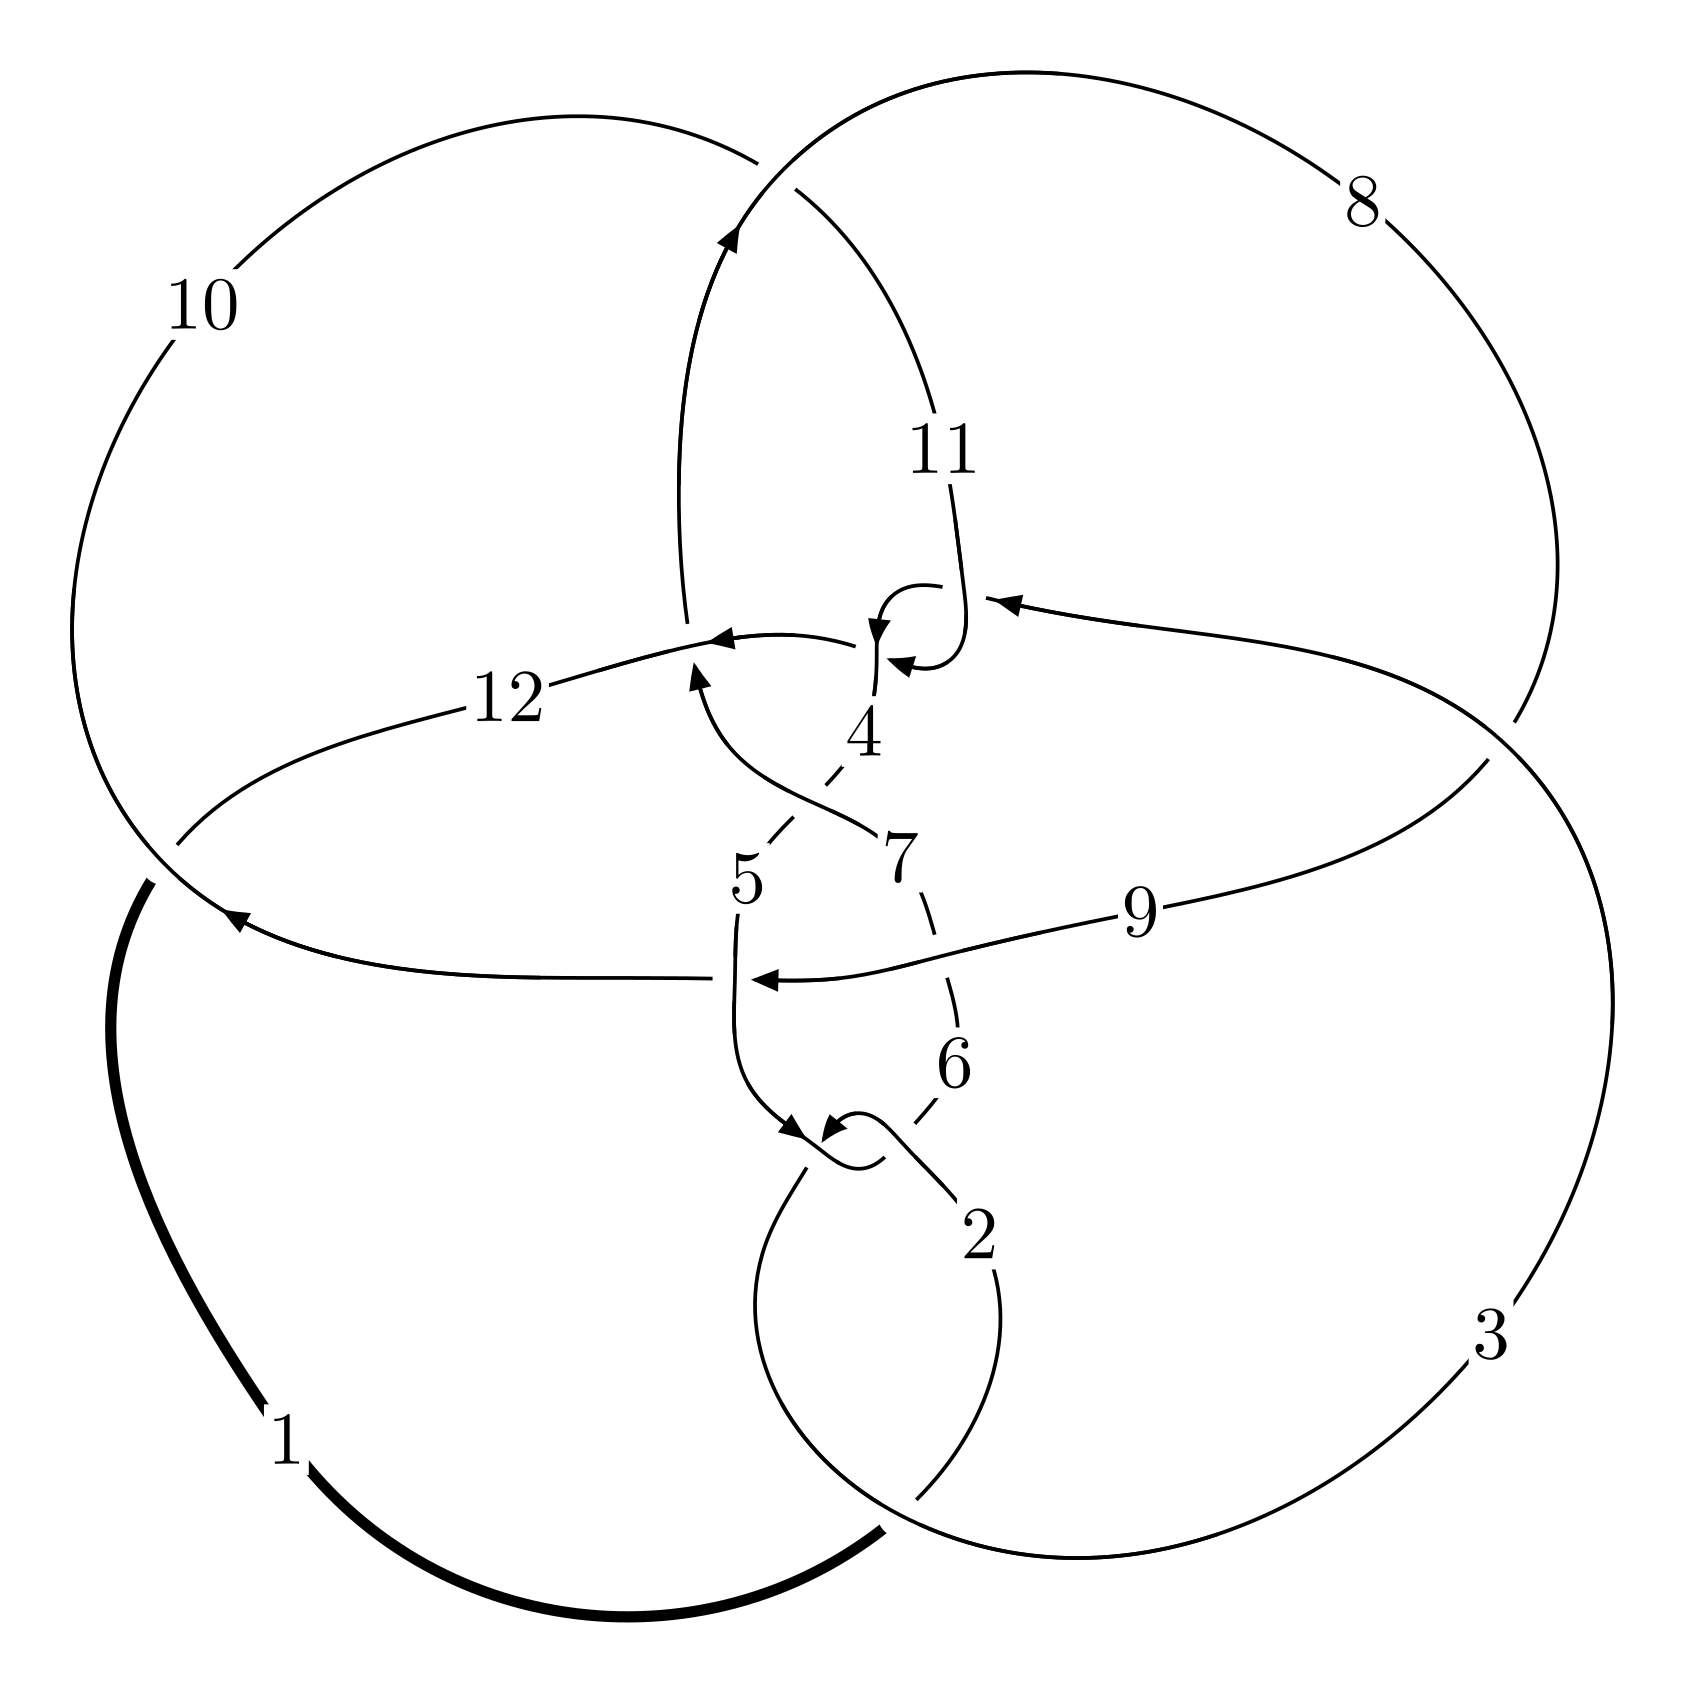
\includegraphics[width=112pt]{../../../GIT/diagram.site/Diagrams/png/2596_12n_0507.png}\\
\ \ \ A knot diagram\footnotemark}&
\allowdisplaybreaks
\textbf{Linearized knot diagam} \\
\cline{2-2}
 &
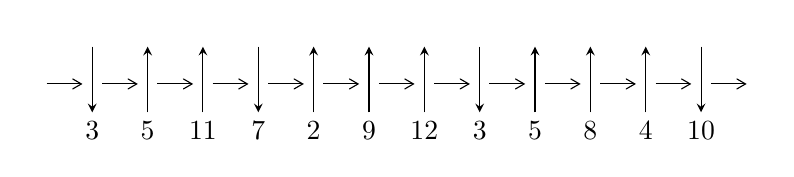
\begin{tikzpicture}[x=20pt, y=17pt]
	% nodes
	\node (C0) at (0, 0) {};
	\node (C1) at (1, 0) {};
	\node (C1U) at (1, +1) {};
	\node (C1D) at (1, -1) {3};

	\node (C2) at (2, 0) {};
	\node (C2U) at (2, +1) {};
	\node (C2D) at (2, -1) {5};

	\node (C3) at (3, 0) {};
	\node (C3U) at (3, +1) {};
	\node (C3D) at (3, -1) {11};

	\node (C4) at (4, 0) {};
	\node (C4U) at (4, +1) {};
	\node (C4D) at (4, -1) {7};

	\node (C5) at (5, 0) {};
	\node (C5U) at (5, +1) {};
	\node (C5D) at (5, -1) {2};

	\node (C6) at (6, 0) {};
	\node (C6U) at (6, +1) {};
	\node (C6D) at (6, -1) {9};

	\node (C7) at (7, 0) {};
	\node (C7U) at (7, +1) {};
	\node (C7D) at (7, -1) {12};

	\node (C8) at (8, 0) {};
	\node (C8U) at (8, +1) {};
	\node (C8D) at (8, -1) {3};

	\node (C9) at (9, 0) {};
	\node (C9U) at (9, +1) {};
	\node (C9D) at (9, -1) {5};

	\node (C10) at (10, 0) {};
	\node (C10U) at (10, +1) {};
	\node (C10D) at (10, -1) {8};

	\node (C11) at (11, 0) {};
	\node (C11U) at (11, +1) {};
	\node (C11D) at (11, -1) {4};

	\node (C12) at (12, 0) {};
	\node (C12U) at (12, +1) {};
	\node (C12D) at (12, -1) {10};
	\node (C13) at (13, 0) {};

	% arrows
	\draw[->,>={angle 60}]
	(C0) edge (C1) (C1) edge (C2) (C2) edge (C3) (C3) edge (C4) (C4) edge (C5) (C5) edge (C6) (C6) edge (C7) (C7) edge (C8) (C8) edge (C9) (C9) edge (C10) (C10) edge (C11) (C11) edge (C12) (C12) edge (C13) ;	\draw[->,>=stealth]
	(C1U) edge (C1D) (C2D) edge (C2U) (C3D) edge (C3U) (C4U) edge (C4D) (C5D) edge (C5U) (C6D) edge (C6U) (C7D) edge (C7U) (C8U) edge (C8D) (C9D) edge (C9U) (C10D) edge (C10U) (C11D) edge (C11U) (C12U) edge (C12D) ;
	\end{tikzpicture} \\
\hhline{~~} \\& 
\textbf{Solving Sequence} \\ \cline{2-2} 
 &
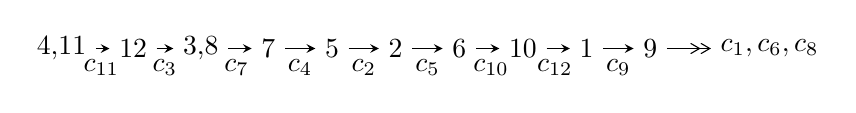
\begin{tikzpicture}[x=23pt, y=7pt]
	% node
	\node (A0) at (-1/8, 0) {4,11};
	\node (A1) at (1, 0) {12};
	\node (A2) at (33/16, 0) {3,8};
	\node (A3) at (25/8, 0) {7};
	\node (A4) at (33/8, 0) {5};
	\node (A5) at (41/8, 0) {2};
	\node (A6) at (49/8, 0) {6};
	\node (A7) at (57/8, 0) {10};
	\node (A8) at (65/8, 0) {1};
	\node (A9) at (73/8, 0) {9};
	\node (C1) at (1/2, -1) {$c_{11}$};
	\node (C2) at (3/2, -1) {$c_{3}$};
	\node (C3) at (21/8, -1) {$c_{7}$};
	\node (C4) at (29/8, -1) {$c_{4}$};
	\node (C5) at (37/8, -1) {$c_{2}$};
	\node (C6) at (45/8, -1) {$c_{5}$};
	\node (C7) at (53/8, -1) {$c_{10}$};
	\node (C8) at (61/8, -1) {$c_{12}$};
	\node (C9) at (69/8, -1) {$c_{9}$};
	\node (A10) at (11, 0) {$c_{1},c_{6},c_{8}$};

	% edge
	\draw[->,>=stealth]	
	(A0) edge (A1) (A1) edge (A2) (A2) edge (A3) (A3) edge (A4) (A4) edge (A5) (A5) edge (A6) (A6) edge (A7) (A7) edge (A8) (A8) edge (A9) ;
	\draw[->>,>={angle 60}]	
	(A9) edge (A10);
\end{tikzpicture} \\ 

\end{tabular} \\

\footnotetext{
The image of knot diagram is generated by the software ``\textbf{Draw programme}" developed by Andrew Bartholomew(\url{http://www.layer8.co.uk/maths/draw/index.htm\#Running-draw}), where we modified some parts for our purpose(\url{https://github.com/CATsTAILs/LinksPainter}).
}\phantom \\ \newline 
\centering \textbf{Ideals for irreducible components\footnotemark of $X_{\text{par}}$} 
 
\begin{align*}
I^u_{1}&=\langle 
1.00284\times10^{74} u^{51}-5.06570\times10^{74} u^{50}+\cdots+2.45946\times10^{74} b-5.12443\times10^{75},\\
\phantom{I^u_{1}}&\phantom{= \langle  }1.96421\times10^{74} u^{51}-1.03477\times10^{75} u^{50}+\cdots+5.81327\times10^{74} a-1.34829\times10^{76},\\
\phantom{I^u_{1}}&\phantom{= \langle  }u^{52}-6 u^{51}+\cdots-168 u+52\rangle \\
I^u_{2}&=\langle 
117054 u^{17}-360970 u^{16}+\cdots+246977 b+230480,\\
\phantom{I^u_{2}}&\phantom{= \langle  }207914 u^{17}-537859 u^{16}+\cdots+740931 a-581924,\;u^{18}-2 u^{17}+\cdots+8 u+3\rangle \\
I^u_{3}&=\langle 
7 a^4+16 a^3-4 a^2+11 b-40 a+8,\;a^5+2 a^4- a^3-6 a^2+3 a-1,\;u+1\rangle \\
\\
I^v_{1}&=\langle 
a,\;b^2- b+1,\;v-1\rangle \\
\end{align*}
\raggedright * 4 irreducible components of $\dim_{\mathbb{C}}=0$, with total 77 representations.\\
\footnotetext{All coefficients of polynomials are rational numbers. But the coefficients are sometimes approximated in decimal forms when there is not enough margin.}
\newpage
\renewcommand{\arraystretch}{1}
\centering \section*{I. $I^u_{1}= \langle 1.00\times10^{74} u^{51}-5.07\times10^{74} u^{50}+\cdots+2.46\times10^{74} b-5.12\times10^{75},\;1.96\times10^{74} u^{51}-1.03\times10^{75} u^{50}+\cdots+5.81\times10^{74} a-1.35\times10^{76},\;u^{52}-6 u^{51}+\cdots-168 u+52 \rangle$}
\flushleft \textbf{(i) Arc colorings}\\
\begin{tabular}{m{7pt} m{180pt} m{7pt} m{180pt} }
\flushright $a_{4}=$&$\begin{pmatrix}0\\u\end{pmatrix}$ \\
\flushright $a_{11}=$&$\begin{pmatrix}1\\0\end{pmatrix}$ \\
\flushright $a_{12}=$&$\begin{pmatrix}1\\- u^2\end{pmatrix}$ \\
\flushright $a_{3}=$&$\begin{pmatrix}- u\\u\end{pmatrix}$ \\
\flushright $a_{8}=$&$\begin{pmatrix}-0.337885 u^{51}+1.78002 u^{50}+\cdots-47.5713 u+23.1933\\-0.407746 u^{51}+2.05968 u^{50}+\cdots-49.5998 u+20.8356\end{pmatrix}$ \\
\flushright $a_{7}=$&$\begin{pmatrix}0.231416 u^{51}-1.16982 u^{50}+\cdots+26.0026 u-10.5013\\-0.746564 u^{51}+3.90831 u^{50}+\cdots-98.2781 u+45.0657\end{pmatrix}$ \\
\flushright $a_{5}=$&$\begin{pmatrix}-0.483569 u^{51}+2.46254 u^{50}+\cdots-59.1117 u+30.0174\\-0.138554 u^{51}+0.761537 u^{50}+\cdots-19.4741 u+10.6533\end{pmatrix}$ \\
\flushright $a_{2}=$&$\begin{pmatrix}0.136698 u^{51}-0.735393 u^{50}+\cdots+21.0106 u-6.84353\\0.189414 u^{51}-0.720852 u^{50}+\cdots+9.10899 u+1.55169\end{pmatrix}$ \\
\flushright $a_{6}=$&$\begin{pmatrix}-0.924358 u^{51}+4.32805 u^{50}+\cdots-89.5677 u+26.2032\\2.94505 u^{51}-14.5616 u^{50}+\cdots+329.171 u-146.279\end{pmatrix}$ \\
\flushright $a_{10}=$&$\begin{pmatrix}-0.558793 u^{51}+2.71369 u^{50}+\cdots-59.1474 u+26.7302\\0.449141 u^{51}-2.26958 u^{50}+\cdots+53.1092 u-22.9509\end{pmatrix}$ \\
\flushright $a_{1}=$&$\begin{pmatrix}0.805085 u^{51}-3.90019 u^{50}+\cdots+88.1248 u-32.8658\\-0.478973 u^{51}+2.44395 u^{50}+\cdots-58.0052 u+27.5740\end{pmatrix}$ \\
\flushright $a_{9}=$&$\begin{pmatrix}0.161202 u^{51}-0.874376 u^{50}+\cdots+20.1820 u-9.77912\\-0.906833 u^{51}+4.71408 u^{50}+\cdots-117.353 u+53.8080\end{pmatrix}$\\&\end{tabular}
\flushleft \textbf{(ii) Obstruction class $= -1$}\\~\\
\flushleft \textbf{(iii) Cusp Shapes $= -1.43996 u^{51}+6.82741 u^{50}+\cdots-140.681 u+61.5443$}\\~\\
\newpage\renewcommand{\arraystretch}{1}
\flushleft \textbf{(iv) u-Polynomials at the component}\newline \\
\begin{tabular}{m{50pt}|m{274pt}}
Crossings & \hspace{64pt}u-Polynomials at each crossing \\
\hline $$\begin{aligned}c_{1}\end{aligned}$$&$\begin{aligned}
&u^{52}+79 u^{51}+\cdots+126 u+1
\end{aligned}$\\
\hline $$\begin{aligned}c_{2},c_{5}\end{aligned}$$&$\begin{aligned}
&u^{52}+u^{51}+\cdots-16 u+1
\end{aligned}$\\
\hline $$\begin{aligned}c_{3},c_{11}\end{aligned}$$&$\begin{aligned}
&u^{52}+6 u^{51}+\cdots+168 u+52
\end{aligned}$\\
\hline $$\begin{aligned}c_{4}\end{aligned}$$&$\begin{aligned}
&u^{52}-7 u^{51}+\cdots-729 u+449
\end{aligned}$\\
\hline $$\begin{aligned}c_{6}\end{aligned}$$&$\begin{aligned}
&u^{52}- u^{51}+\cdots-32223752 u+2811556
\end{aligned}$\\
\hline $$\begin{aligned}c_{7}\end{aligned}$$&$\begin{aligned}
&u^{52}-3 u^{51}+\cdots-97 u+49
\end{aligned}$\\
\hline $$\begin{aligned}c_{8}\end{aligned}$$&$\begin{aligned}
&u^{52}- u^{51}+\cdots-248316 u+85849
\end{aligned}$\\
\hline $$\begin{aligned}c_{9}\end{aligned}$$&$\begin{aligned}
&u^{52}-2 u^{51}+\cdots+172169 u+39973
\end{aligned}$\\
\hline $$\begin{aligned}c_{10}\end{aligned}$$&$\begin{aligned}
&u^{52}+11 u^{51}+\cdots+560 u+49
\end{aligned}$\\
\hline $$\begin{aligned}c_{12}\end{aligned}$$&$\begin{aligned}
&u^{52}-15 u^{51}+\cdots-112029 u+100799
\end{aligned}$\\
\hline
\end{tabular}\\~\\
\newpage\renewcommand{\arraystretch}{1}
\flushleft \textbf{(v) Riley Polynomials at the component}\newline \\
\begin{tabular}{m{50pt}|m{274pt}}
Crossings & \hspace{64pt}Riley Polynomials at each crossing \\
\hline $$\begin{aligned}c_{1}\end{aligned}$$&$\begin{aligned}
&y^{52}-209 y^{51}+\cdots+2042 y+1
\end{aligned}$\\
\hline $$\begin{aligned}c_{2},c_{5}\end{aligned}$$&$\begin{aligned}
&y^{52}+79 y^{51}+\cdots+126 y+1
\end{aligned}$\\
\hline $$\begin{aligned}c_{3},c_{11}\end{aligned}$$&$\begin{aligned}
&y^{52}-40 y^{51}+\cdots-11792 y+2704
\end{aligned}$\\
\hline $$\begin{aligned}c_{4}\end{aligned}$$&$\begin{aligned}
&y^{52}+27 y^{51}+\cdots+5239107 y+201601
\end{aligned}$\\
\hline $$\begin{aligned}c_{6}\end{aligned}$$&$\begin{aligned}
&y^{52}+93 y^{51}+\cdots-26572892374864 y+7904847141136
\end{aligned}$\\
\hline $$\begin{aligned}c_{7}\end{aligned}$$&$\begin{aligned}
&y^{52}-15 y^{51}+\cdots-35575 y+2401
\end{aligned}$\\
\hline $$\begin{aligned}c_{8}\end{aligned}$$&$\begin{aligned}
&y^{52}-15 y^{51}+\cdots-75223432574 y+7370050801
\end{aligned}$\\
\hline $$\begin{aligned}c_{9}\end{aligned}$$&$\begin{aligned}
&y^{52}+80 y^{51}+\cdots+24550030999 y+1597840729
\end{aligned}$\\
\hline $$\begin{aligned}c_{10}\end{aligned}$$&$\begin{aligned}
&y^{52}+7 y^{51}+\cdots+23618 y+2401
\end{aligned}$\\
\hline $$\begin{aligned}c_{12}\end{aligned}$$&$\begin{aligned}
&y^{52}-45 y^{51}+\cdots+108799403279 y+10160438401
\end{aligned}$\\
\hline
\end{tabular}\\~\\
\newpage\flushleft \textbf{(vi) Complex Volumes and Cusp Shapes}
$$\begin{array}{c|c|c}  
\text{Solutions to }I^u_{1}& \I (\text{vol} + \sqrt{-1}CS) & \text{Cusp shape}\\
 \hline 
\begin{aligned}
u &= -0.072076 + 1.073670 I \\
a &= \phantom{-}0.422821 + 0.107445 I \\
b &= -0.157151 + 0.717710 I\end{aligned}
 & -0.08598 - 3.46440 I & \phantom{-0.000000 -}0. + 3.76930 I \\ \hline\begin{aligned}
u &= -0.072076 - 1.073670 I \\
a &= \phantom{-}0.422821 - 0.107445 I \\
b &= -0.157151 - 0.717710 I\end{aligned}
 & -0.08598 + 3.46440 I & \phantom{-0.000000 } 0. - 3.76930 I \\ \hline\begin{aligned}
u &= \phantom{-}1.068700 + 0.176322 I \\
a &= \phantom{-}0.99400 - 1.18957 I \\
b &= -0.471542 - 1.119630 I\end{aligned}
 & -7.77272 + 4.78722 I & \phantom{-}5.62286 - 4.46937 I \\ \hline\begin{aligned}
u &= \phantom{-}1.068700 - 0.176322 I \\
a &= \phantom{-}0.99400 + 1.18957 I \\
b &= -0.471542 + 1.119630 I\end{aligned}
 & -7.77272 - 4.78722 I & \phantom{-}5.62286 + 4.46937 I \\ \hline\begin{aligned}
u &= -0.269878 + 0.867397 I \\
a &= -0.065611 - 0.173550 I \\
b &= \phantom{-}0.680688 - 0.688393 I\end{aligned}
 & \phantom{-}0.88668 - 2.29079 I & \phantom{-}4.46889 + 2.66895 I \\ \hline\begin{aligned}
u &= -0.269878 - 0.867397 I \\
a &= -0.065611 + 0.173550 I \\
b &= \phantom{-}0.680688 + 0.688393 I\end{aligned}
 & \phantom{-}0.88668 + 2.29079 I & \phantom{-}4.46889 - 2.66895 I \\ \hline\begin{aligned}
u &= \phantom{-}1.048260 + 0.371285 I \\
a &= \phantom{-}1.55261 + 0.09090 I \\
b &= -0.733122 - 0.676797 I\end{aligned}
 & -0.94506 + 3.54563 I & \phantom{-}1.62965 - 5.75409 I \\ \hline\begin{aligned}
u &= \phantom{-}1.048260 - 0.371285 I \\
a &= \phantom{-}1.55261 - 0.09090 I \\
b &= -0.733122 + 0.676797 I\end{aligned}
 & -0.94506 - 3.54563 I & \phantom{-}1.62965 + 5.75409 I \\ \hline\begin{aligned}
u &= \phantom{-}1.104730 + 0.182136 I \\
a &= \phantom{-}0.839035 - 0.685937 I \\
b &= -0.615619 + 1.264700 I\end{aligned}
 & \phantom{-}3.12675 + 4.09577 I & \phantom{-}11.1869 - 8.8133 I \\ \hline\begin{aligned}
u &= \phantom{-}1.104730 - 0.182136 I \\
a &= \phantom{-}0.839035 + 0.685937 I \\
b &= -0.615619 - 1.264700 I\end{aligned}
 & \phantom{-}3.12675 - 4.09577 I & \phantom{-}11.1869 + 8.8133 I\\
 \hline 
 \end{array}$$\newpage$$\begin{array}{c|c|c}  
\text{Solutions to }I^u_{1}& \I (\text{vol} + \sqrt{-1}CS) & \text{Cusp shape}\\
 \hline 
\begin{aligned}
u &= -1.132840 + 0.177320 I \\
a &= -1.42486 + 0.17109 I \\
b &= \phantom{-}1.32434 - 1.18522 I\end{aligned}
 & \phantom{-}2.29045 - 1.02276 I & \phantom{-}4.00000 + 0. I\phantom{ +0.000000I} \\ \hline\begin{aligned}
u &= -1.132840 - 0.177320 I \\
a &= -1.42486 - 0.17109 I \\
b &= \phantom{-}1.32434 + 1.18522 I\end{aligned}
 & \phantom{-}2.29045 + 1.02276 I & \phantom{-}4.00000 + 0. I\phantom{ +0.000000I} \\ \hline\begin{aligned}
u &= -0.280215 + 0.778839 I \\
a &= -0.567039 + 0.203024 I \\
b &= -0.80247 - 1.29034 I\end{aligned}
 & -12.44140 + 2.96434 I & -0.898916 - 0.509328 I \\ \hline\begin{aligned}
u &= -0.280215 - 0.778839 I \\
a &= -0.567039 - 0.203024 I \\
b &= -0.80247 + 1.29034 I\end{aligned}
 & -12.44140 - 2.96434 I & -0.898916 + 0.509328 I \\ \hline\begin{aligned}
u &= \phantom{-}0.495944 + 0.659946 I \\
a &= -0.93403 + 1.16897 I \\
b &= -0.782553 + 0.575131 I\end{aligned}
 & -8.85362 + 2.74417 I & \phantom{-}1.62020 - 2.60444 I \\ \hline\begin{aligned}
u &= \phantom{-}0.495944 - 0.659946 I \\
a &= -0.93403 - 1.16897 I \\
b &= -0.782553 - 0.575131 I\end{aligned}
 & -8.85362 - 2.74417 I & \phantom{-}1.62020 + 2.60444 I \\ \hline\begin{aligned}
u &= \phantom{-}0.383796 + 0.722249 I \\
a &= \phantom{-}0.0394551 + 0.0110081 I \\
b &= -0.141872 + 0.858570 I\end{aligned}
 & -3.00681 + 0.54202 I & -3.07092 - 1.78302 I \\ \hline\begin{aligned}
u &= \phantom{-}0.383796 - 0.722249 I \\
a &= \phantom{-}0.0394551 - 0.0110081 I \\
b &= -0.141872 - 0.858570 I\end{aligned}
 & -3.00681 - 0.54202 I & -3.07092 + 1.78302 I \\ \hline\begin{aligned}
u &= -1.118520 + 0.405885 I \\
a &= -1.99263 - 0.26808 I \\
b &= \phantom{-}0.607693 - 0.824065 I\end{aligned}
 & \phantom{-}2.47983 - 5.59777 I & \phantom{-0.000000 -}0. + 7.04199 I \\ \hline\begin{aligned}
u &= -1.118520 - 0.405885 I \\
a &= -1.99263 + 0.26808 I \\
b &= \phantom{-}0.607693 + 0.824065 I\end{aligned}
 & \phantom{-}2.47983 + 5.59777 I & \phantom{-0.000000 } 0. - 7.04199 I\\
 \hline 
 \end{array}$$\newpage$$\begin{array}{c|c|c}  
\text{Solutions to }I^u_{1}& \I (\text{vol} + \sqrt{-1}CS) & \text{Cusp shape}\\
 \hline 
\begin{aligned}
u &= \phantom{-}0.989819 + 0.690556 I \\
a &= \phantom{-}0.738252 - 1.108280 I \\
b &= -0.493528 - 1.071940 I\end{aligned}
 & -7.62938 + 2.46347 I & \phantom{-0.000000 } 0 \\ \hline\begin{aligned}
u &= \phantom{-}0.989819 - 0.690556 I \\
a &= \phantom{-}0.738252 + 1.108280 I \\
b &= -0.493528 + 1.071940 I\end{aligned}
 & -7.62938 - 2.46347 I & \phantom{-0.000000 } 0 \\ \hline\begin{aligned}
u &= \phantom{-}1.209340 + 0.050765 I \\
a &= -1.57890 - 0.62627 I \\
b &= \phantom{-}1.37163 + 1.27972 I\end{aligned}
 & \phantom{-}5.14318 + 1.81368 I & \phantom{-}18.0333 + 0. I\phantom{ +0.000000I} \\ \hline\begin{aligned}
u &= \phantom{-}1.209340 - 0.050765 I \\
a &= -1.57890 + 0.62627 I \\
b &= \phantom{-}1.37163 - 1.27972 I\end{aligned}
 & \phantom{-}5.14318 - 1.81368 I & \phantom{-}18.0333 + 0. I\phantom{ +0.000000I} \\ \hline\begin{aligned}
u &= -1.142540 + 0.409057 I \\
a &= \phantom{-}1.98363 - 0.31458 I \\
b &= -1.28875 + 1.59470 I\end{aligned}
 & -9.77699 - 7.32778 I & \phantom{-0.000000 } 0 \\ \hline\begin{aligned}
u &= -1.142540 - 0.409057 I \\
a &= \phantom{-}1.98363 + 0.31458 I \\
b &= -1.28875 - 1.59470 I\end{aligned}
 & -9.77699 + 7.32778 I & \phantom{-0.000000 } 0 \\ \hline\begin{aligned}
u &= \phantom{-}0.038697 + 1.225180 I \\
a &= \phantom{-}0.060632 - 0.219112 I \\
b &= -0.787773 - 1.095970 I\end{aligned}
 & -10.30200 + 8.83554 I & \phantom{-0.000000 } 0 \\ \hline\begin{aligned}
u &= \phantom{-}0.038697 - 1.225180 I \\
a &= \phantom{-}0.060632 + 0.219112 I \\
b &= -0.787773 + 1.095970 I\end{aligned}
 & -10.30200 - 8.83554 I & \phantom{-0.000000 } 0 \\ \hline\begin{aligned}
u &= -1.298120 + 0.219749 I \\
a &= \phantom{-}1.57172 + 0.70746 I \\
b &= -2.01283 - 0.85764 I\end{aligned}
 & -3.60868 - 5.39855 I & \phantom{-0.000000 } 0 \\ \hline\begin{aligned}
u &= -1.298120 - 0.219749 I \\
a &= \phantom{-}1.57172 - 0.70746 I \\
b &= -2.01283 + 0.85764 I\end{aligned}
 & -3.60868 + 5.39855 I & \phantom{-0.000000 } 0\\
 \hline 
 \end{array}$$\newpage$$\begin{array}{c|c|c}  
\text{Solutions to }I^u_{1}& \I (\text{vol} + \sqrt{-1}CS) & \text{Cusp shape}\\
 \hline 
\begin{aligned}
u &= -0.435814 + 0.497980 I \\
a &= -0.144770 + 1.329400 I \\
b &= \phantom{-}0.406646 + 0.837607 I\end{aligned}
 & \phantom{-}0.35496 + 1.82856 I & \phantom{-}2.55368 - 2.81717 I \\ \hline\begin{aligned}
u &= -0.435814 - 0.497980 I \\
a &= -0.144770 - 1.329400 I \\
b &= \phantom{-}0.406646 - 0.837607 I\end{aligned}
 & \phantom{-}0.35496 - 1.82856 I & \phantom{-}2.55368 + 2.81717 I \\ \hline\begin{aligned}
u &= -1.325900 + 0.415407 I \\
a &= \phantom{-}1.133880 + 0.064846 I \\
b &= -0.593152 + 0.351949 I\end{aligned}
 & \phantom{-}5.15254 - 2.08012 I & \phantom{-0.000000 } 0 \\ \hline\begin{aligned}
u &= -1.325900 - 0.415407 I \\
a &= \phantom{-}1.133880 - 0.064846 I \\
b &= -0.593152 - 0.351949 I\end{aligned}
 & \phantom{-}5.15254 + 2.08012 I & \phantom{-0.000000 } 0 \\ \hline\begin{aligned}
u &= \phantom{-}0.594624 + 0.117518 I \\
a &= -2.93422 - 1.82812 I \\
b &= -0.610865 + 0.355975 I\end{aligned}
 & -9.27919 - 3.18450 I & \phantom{-}2.07898 - 0.42481 I \\ \hline\begin{aligned}
u &= \phantom{-}0.594624 - 0.117518 I \\
a &= -2.93422 + 1.82812 I \\
b &= -0.610865 - 0.355975 I\end{aligned}
 & -9.27919 + 3.18450 I & \phantom{-}2.07898 + 0.42481 I \\ \hline\begin{aligned}
u &= \phantom{-}1.34204 + 0.52912 I \\
a &= \phantom{-}1.308500 - 0.013301 I \\
b &= -0.646221 - 0.811256 I\end{aligned}
 & \phantom{-}4.19597 + 9.10494 I & \phantom{-0.000000 } 0 \\ \hline\begin{aligned}
u &= \phantom{-}1.34204 - 0.52912 I \\
a &= \phantom{-}1.308500 + 0.013301 I \\
b &= -0.646221 + 0.811256 I\end{aligned}
 & \phantom{-}4.19597 - 9.10494 I & \phantom{-0.000000 } 0 \\ \hline\begin{aligned}
u &= \phantom{-}1.38606 + 0.43784 I \\
a &= -1.47210 - 0.00392 I \\
b &= \phantom{-}1.21303 + 1.00411 I\end{aligned}
 & \phantom{-}5.90548 + 7.10957 I & \phantom{-0.000000 } 0 \\ \hline\begin{aligned}
u &= \phantom{-}1.38606 - 0.43784 I \\
a &= -1.47210 + 0.00392 I \\
b &= \phantom{-}1.21303 - 1.00411 I\end{aligned}
 & \phantom{-}5.90548 - 7.10957 I & \phantom{-0.000000 } 0\\
 \hline 
 \end{array}$$\newpage$$\begin{array}{c|c|c}  
\text{Solutions to }I^u_{1}& \I (\text{vol} + \sqrt{-1}CS) & \text{Cusp shape}\\
 \hline 
\begin{aligned}
u &= \phantom{-}0.163645 + 0.500729 I \\
a &= \phantom{-}1.48155 - 0.11869 I \\
b &= -0.210860 - 0.434892 I\end{aligned}
 & \phantom{-}0.61514 - 1.70536 I & \phantom{-}3.89799 + 3.77276 I \\ \hline\begin{aligned}
u &= \phantom{-}0.163645 - 0.500729 I \\
a &= \phantom{-}1.48155 + 0.11869 I \\
b &= -0.210860 + 0.434892 I\end{aligned}
 & \phantom{-}0.61514 + 1.70536 I & \phantom{-}3.89799 - 3.77276 I \\ \hline\begin{aligned}
u &= -1.40514 + 0.56979 I \\
a &= \phantom{-}1.50502 - 0.02569 I \\
b &= -1.02860 + 1.37422 I\end{aligned}
 & -5.7801 - 15.0850 I & \phantom{-0.000000 } 0 \\ \hline\begin{aligned}
u &= -1.40514 - 0.56979 I \\
a &= \phantom{-}1.50502 + 0.02569 I \\
b &= -1.02860 - 1.37422 I\end{aligned}
 & -5.7801 + 15.0850 I & \phantom{-0.000000 } 0 \\ \hline\begin{aligned}
u &= -0.334164 + 0.327190 I \\
a &= \phantom{-}0.80947 - 1.27346 I \\
b &= \phantom{-}0.454762 - 0.337305 I\end{aligned}
 & \phantom{-}0.700125 - 1.067100 I & \phantom{-}7.65429 + 6.43905 I \\ \hline\begin{aligned}
u &= -0.334164 - 0.327190 I \\
a &= \phantom{-}0.80947 + 1.27346 I \\
b &= \phantom{-}0.454762 + 0.337305 I\end{aligned}
 & \phantom{-}0.700125 + 1.067100 I & \phantom{-}7.65429 - 6.43905 I \\ \hline\begin{aligned}
u &= -1.54216 + 0.53974 I \\
a &= -0.817027 + 0.067290 I \\
b &= \phantom{-}0.805620 - 0.732243 I\end{aligned}
 & \phantom{-}4.04363 - 5.57601 I & \phantom{-0.000000 } 0 \\ \hline\begin{aligned}
u &= -1.54216 - 0.53974 I \\
a &= -0.817027 - 0.067290 I \\
b &= \phantom{-}0.805620 + 0.732243 I\end{aligned}
 & \phantom{-}4.04363 + 5.57601 I & \phantom{-0.000000 } 0 \\ \hline\begin{aligned}
u &= \phantom{-}1.82542 + 0.12353 I \\
a &= \phantom{-}0.180716 - 0.464332 I \\
b &= -0.529222 + 0.477306 I\end{aligned}
 & -5.59317 + 0.61259 I & \phantom{-0.000000 } 0 \\ \hline\begin{aligned}
u &= \phantom{-}1.82542 - 0.12353 I \\
a &= \phantom{-}0.180716 + 0.464332 I \\
b &= -0.529222 - 0.477306 I\end{aligned}
 & -5.59317 - 0.61259 I & \phantom{-0.000000 } 0\\
 \hline 
 \end{array}$$\newpage$$\begin{array}{c|c|c}  
\text{Solutions to }I^u_{1}& \I (\text{vol} + \sqrt{-1}CS) & \text{Cusp shape}\\
 \hline 
\begin{aligned}
u &= \phantom{-}1.70629 + 0.88313 I \\
a &= \phantom{-}0.040681 - 0.244589 I \\
b &= -0.458284 + 0.504879 I\end{aligned}
 & -5.74740 - 1.53118 I & \phantom{-0.000000 } 0 \\ \hline\begin{aligned}
u &= \phantom{-}1.70629 - 0.88313 I \\
a &= \phantom{-}0.040681 + 0.244589 I \\
b &= -0.458284 - 0.504879 I\end{aligned}
 & -5.74740 + 1.53118 I & \phantom{-0.000000 } 0\\
 \hline 
 \end{array}$$\newpage\newpage\renewcommand{\arraystretch}{1}
\centering \section*{II. $I^u_{2}= \langle 1.17\times10^{5} u^{17}-3.61\times10^{5} u^{16}+\cdots+2.47\times10^{5} b+2.30\times10^{5},\;2.08\times10^{5} u^{17}-5.38\times10^{5} u^{16}+\cdots+7.41\times10^{5} a-5.82\times10^{5},\;u^{18}-2 u^{17}+\cdots+8 u+3 \rangle$}
\flushleft \textbf{(i) Arc colorings}\\
\begin{tabular}{m{7pt} m{180pt} m{7pt} m{180pt} }
\flushright $a_{4}=$&$\begin{pmatrix}0\\u\end{pmatrix}$ \\
\flushright $a_{11}=$&$\begin{pmatrix}1\\0\end{pmatrix}$ \\
\flushright $a_{12}=$&$\begin{pmatrix}1\\- u^2\end{pmatrix}$ \\
\flushright $a_{3}=$&$\begin{pmatrix}- u\\u\end{pmatrix}$ \\
\flushright $a_{8}=$&$\begin{pmatrix}-0.280612 u^{17}+0.725923 u^{16}+\cdots-3.10639 u+0.785396\\-0.473947 u^{17}+1.46155 u^{16}+\cdots-2.24939 u-0.933204\end{pmatrix}$ \\
\flushright $a_{7}=$&$\begin{pmatrix}0.237918 u^{17}-0.825679 u^{16}+\cdots-0.381241 u+2.21270\\-0.894460 u^{17}+2.94986 u^{16}+\cdots-4.81013 u-2.47683\end{pmatrix}$ \\
\flushright $a_{5}=$&$\begin{pmatrix}-0.605086 u^{17}+1.13512 u^{16}+\cdots-3.56873 u-1.00410\\0.513671 u^{17}-0.344639 u^{16}+\cdots-4.46092 u-1.91207\end{pmatrix}$ \\
\flushright $a_{2}=$&$\begin{pmatrix}0.758081 u^{17}-1.12381 u^{16}+\cdots-3.30368 u-1.75050\\-0.800844 u^{17}+1.20535 u^{16}+\cdots+9.72215 u+2.40419\end{pmatrix}$ \\
\flushright $a_{6}=$&$\begin{pmatrix}-0.210071 u^{17}+1.20477 u^{16}+\cdots-7.21760 u-1.54346\\-0.623933 u^{17}+0.206902 u^{16}+\cdots+7.78891 u+2.25446\end{pmatrix}$ \\
\flushright $a_{10}=$&$\begin{pmatrix}-0.457344 u^{17}-0.485917 u^{16}+\cdots+1.87185 u+1.65301\\0.188467 u^{17}+1.56389 u^{16}+\cdots-12.1388 u-4.59404\end{pmatrix}$ \\
\flushright $a_{1}=$&$\begin{pmatrix}0.852110 u^{17}-1.08511 u^{16}+\cdots-3.14348 u-1.73854\\-0.894873 u^{17}+1.16664 u^{16}+\cdots+9.56196 u+2.39223\end{pmatrix}$ \\
\flushright $a_{9}=$&$\begin{pmatrix}0.132791 u^{17}-0.992322 u^{16}+\cdots+0.0568042 u+2.82047\\-0.887350 u^{17}+3.17980 u^{16}+\cdots-5.41258 u-2.96828\end{pmatrix}$\\&\end{tabular}
\flushleft \textbf{(ii) Obstruction class $= 1$}\\~\\
\flushleft \textbf{(iii) Cusp Shapes $= \frac{39445}{246977} u^{17}-\frac{1167483}{246977} u^{16}+\cdots+\frac{8666107}{246977} u+\frac{3104388}{246977}$}\\~\\
\newpage\renewcommand{\arraystretch}{1}
\flushleft \textbf{(iv) u-Polynomials at the component}\newline \\
\begin{tabular}{m{50pt}|m{274pt}}
Crossings & \hspace{64pt}u-Polynomials at each crossing \\
\hline $$\begin{aligned}c_{1}\end{aligned}$$&$\begin{aligned}
&u^{18}-21 u^{17}+\cdots-23 u+1
\end{aligned}$\\
\hline $$\begin{aligned}c_{2}\end{aligned}$$&$\begin{aligned}
&u^{18}- u^{17}+\cdots+u+1
\end{aligned}$\\
\hline $$\begin{aligned}c_{3}\end{aligned}$$&$\begin{aligned}
&u^{18}+2 u^{17}+\cdots-8 u+3
\end{aligned}$\\
\hline $$\begin{aligned}c_{4}\end{aligned}$$&$\begin{aligned}
&u^{18}-5 u^{17}+\cdots-10 u+11
\end{aligned}$\\
\hline $$\begin{aligned}c_{5}\end{aligned}$$&$\begin{aligned}
&u^{18}+u^{17}+\cdots- u+1
\end{aligned}$\\
\hline $$\begin{aligned}c_{6}\end{aligned}$$&$\begin{aligned}
&u^{18}+4 u^{17}+\cdots+8 u+3
\end{aligned}$\\
\hline $$\begin{aligned}c_{7}\end{aligned}$$&$\begin{aligned}
&u^{18}-3 u^{17}+\cdots-22 u+5
\end{aligned}$\\
\hline $$\begin{aligned}c_{8}\end{aligned}$$&$\begin{aligned}
&u^{18}- u^{17}+\cdots+u+5
\end{aligned}$\\
\hline $$\begin{aligned}c_{9}\end{aligned}$$&$\begin{aligned}
&u^{18}+5 u^{16}+\cdots-4 u+1
\end{aligned}$\\
\hline $$\begin{aligned}c_{10}\end{aligned}$$&$\begin{aligned}
&u^{18}-9 u^{17}+\cdots- u+1
\end{aligned}$\\
\hline $$\begin{aligned}c_{11}\end{aligned}$$&$\begin{aligned}
&u^{18}-2 u^{17}+\cdots+8 u+3
\end{aligned}$\\
\hline $$\begin{aligned}c_{12}\end{aligned}$$&$\begin{aligned}
&u^{18}-7 u^{17}+\cdots-14 u+11
\end{aligned}$\\
\hline
\end{tabular}\\~\\
\newpage\renewcommand{\arraystretch}{1}
\flushleft \textbf{(v) Riley Polynomials at the component}\newline \\
\begin{tabular}{m{50pt}|m{274pt}}
Crossings & \hspace{64pt}Riley Polynomials at each crossing \\
\hline $$\begin{aligned}c_{1}\end{aligned}$$&$\begin{aligned}
&y^{18}-47 y^{17}+\cdots-89 y+1
\end{aligned}$\\
\hline $$\begin{aligned}c_{2},c_{5}\end{aligned}$$&$\begin{aligned}
&y^{18}+21 y^{17}+\cdots+23 y+1
\end{aligned}$\\
\hline $$\begin{aligned}c_{3},c_{11}\end{aligned}$$&$\begin{aligned}
&y^{18}-20 y^{17}+\cdots-58 y+9
\end{aligned}$\\
\hline $$\begin{aligned}c_{4}\end{aligned}$$&$\begin{aligned}
&y^{18}+9 y^{17}+\cdots+956 y+121
\end{aligned}$\\
\hline $$\begin{aligned}c_{6}\end{aligned}$$&$\begin{aligned}
&y^{18}+18 y^{17}+\cdots+68 y+9
\end{aligned}$\\
\hline $$\begin{aligned}c_{7}\end{aligned}$$&$\begin{aligned}
&y^{18}-5 y^{17}+\cdots-104 y+25
\end{aligned}$\\
\hline $$\begin{aligned}c_{8}\end{aligned}$$&$\begin{aligned}
&y^{18}+7 y^{17}+\cdots+29 y+25
\end{aligned}$\\
\hline $$\begin{aligned}c_{9}\end{aligned}$$&$\begin{aligned}
&y^{18}+10 y^{17}+\cdots-8 y+1
\end{aligned}$\\
\hline $$\begin{aligned}c_{10}\end{aligned}$$&$\begin{aligned}
&y^{18}-3 y^{17}+\cdots+3 y+1
\end{aligned}$\\
\hline $$\begin{aligned}c_{12}\end{aligned}$$&$\begin{aligned}
&y^{18}-15 y^{17}+\cdots+1256 y+121
\end{aligned}$\\
\hline
\end{tabular}\\~\\
\newpage\flushleft \textbf{(vi) Complex Volumes and Cusp Shapes}
$$\begin{array}{c|c|c}  
\text{Solutions to }I^u_{2}& \I (\text{vol} + \sqrt{-1}CS) & \text{Cusp shape}\\
 \hline 
\begin{aligned}
u &= -1.005450 + 0.295263 I \\
a &= \phantom{-}1.203530 + 0.437285 I \\
b &= -0.335827 - 0.487120 I\end{aligned}
 & \phantom{-}2.17303 - 3.53081 I & \phantom{-}4.11221 + 3.61845 I \\ \hline\begin{aligned}
u &= -1.005450 - 0.295263 I \\
a &= \phantom{-}1.203530 - 0.437285 I \\
b &= -0.335827 + 0.487120 I\end{aligned}
 & \phantom{-}2.17303 + 3.53081 I & \phantom{-}4.11221 - 3.61845 I \\ \hline\begin{aligned}
u &= -0.207208 + 0.849001 I \\
a &= -0.282886 + 0.138697 I \\
b &= \phantom{-}0.549633 - 0.563104 I\end{aligned}
 & \phantom{-}1.17142 - 3.80180 I & \phantom{-}6.45298 + 6.93246 I \\ \hline\begin{aligned}
u &= -0.207208 - 0.849001 I \\
a &= -0.282886 - 0.138697 I \\
b &= \phantom{-}0.549633 + 0.563104 I\end{aligned}
 & \phantom{-}1.17142 + 3.80180 I & \phantom{-}6.45298 - 6.93246 I \\ \hline\begin{aligned}
u &= \phantom{-}1.161860 + 0.107310 I \\
a &= -2.23789 - 0.78537 I \\
b &= \phantom{-}2.15942 + 1.58054 I\end{aligned}
 & \phantom{-}3.02525 + 1.29728 I & \phantom{-}13.4543 - 5.0288 I \\ \hline\begin{aligned}
u &= \phantom{-}1.161860 - 0.107310 I \\
a &= -2.23789 + 0.78537 I \\
b &= \phantom{-}2.15942 - 1.58054 I\end{aligned}
 & \phantom{-}3.02525 - 1.29728 I & \phantom{-}13.4543 + 5.0288 I \\ \hline\begin{aligned}
u &= \phantom{-}0.751188 + 0.315078 I \\
a &= \phantom{-}1.51622 - 2.08382 I \\
b &= -0.655881 - 0.938092 I\end{aligned}
 & -9.23443 + 4.41108 I & \phantom{-}1.12625 - 5.00994 I \\ \hline\begin{aligned}
u &= \phantom{-}0.751188 - 0.315078 I \\
a &= \phantom{-}1.51622 + 2.08382 I \\
b &= -0.655881 + 0.938092 I\end{aligned}
 & -9.23443 - 4.41108 I & \phantom{-}1.12625 + 5.00994 I \\ \hline\begin{aligned}
u &= -1.218070 + 0.029447 I \\
a &= -1.184950 + 0.350003 I \\
b &= \phantom{-}0.820578 - 1.114160 I\end{aligned}
 & \phantom{-}4.34167 - 2.03661 I & \phantom{-}7.20835 + 3.90028 I \\ \hline\begin{aligned}
u &= -1.218070 - 0.029447 I \\
a &= -1.184950 - 0.350003 I \\
b &= \phantom{-}0.820578 + 1.114160 I\end{aligned}
 & \phantom{-}4.34167 + 2.03661 I & \phantom{-}7.20835 - 3.90028 I\\
 \hline 
 \end{array}$$\newpage$$\begin{array}{c|c|c}  
\text{Solutions to }I^u_{2}& \I (\text{vol} + \sqrt{-1}CS) & \text{Cusp shape}\\
 \hline 
\begin{aligned}
u &= \phantom{-}1.38134 + 0.46176 I \\
a &= -1.399010 + 0.094856 I \\
b &= \phantom{-}1.182680 + 0.724988 I\end{aligned}
 & \phantom{-}6.00324 + 8.77263 I & \phantom{-}8.55851 - 6.89757 I \\ \hline\begin{aligned}
u &= \phantom{-}1.38134 - 0.46176 I \\
a &= -1.399010 - 0.094856 I \\
b &= \phantom{-}1.182680 - 0.724988 I\end{aligned}
 & \phantom{-}6.00324 - 8.77263 I & \phantom{-}8.55851 + 6.89757 I \\ \hline\begin{aligned}
u &= -1.40929 + 0.49254 I \\
a &= -1.140630 - 0.031844 I \\
b &= \phantom{-}0.703194 - 0.839704 I\end{aligned}
 & \phantom{-}5.15223 - 3.52976 I & \phantom{-}7.05597 + 3.81806 I \\ \hline\begin{aligned}
u &= -1.40929 - 0.49254 I \\
a &= -1.140630 + 0.031844 I \\
b &= \phantom{-}0.703194 + 0.839704 I\end{aligned}
 & \phantom{-}5.15223 + 3.52976 I & \phantom{-}7.05597 - 3.81806 I \\ \hline\begin{aligned}
u &= -0.282235 + 0.273085 I \\
a &= \phantom{-}2.34179 - 1.33257 I \\
b &= \phantom{-}0.414830 - 0.603446 I\end{aligned}
 & -0.0620604 - 0.0079783 I & -0.270726 + 0.542760 I \\ \hline\begin{aligned}
u &= -0.282235 - 0.273085 I \\
a &= \phantom{-}2.34179 + 1.33257 I \\
b &= \phantom{-}0.414830 + 0.603446 I\end{aligned}
 & -0.0620604 + 0.0079783 I & -0.270726 - 0.542760 I \\ \hline\begin{aligned}
u &= \phantom{-}1.82787 + 0.56276 I \\
a &= -0.149506 - 0.193772 I \\
b &= -0.338633 + 0.304616 I\end{aligned}
 & -5.99061 - 1.24449 I & -6.19786 - 0.78651 I \\ \hline\begin{aligned}
u &= \phantom{-}1.82787 - 0.56276 I \\
a &= -0.149506 + 0.193772 I \\
b &= -0.338633 - 0.304616 I\end{aligned}
 & -5.99061 + 1.24449 I & -6.19786 + 0.78651 I\\
 \hline 
 \end{array}$$\newpage\newpage\renewcommand{\arraystretch}{1}
\centering \section*{III. $I^u_{3}= \langle 7 a^4+16 a^3-4 a^2+11 b-40 a+8,\;a^5+2 a^4- a^3-6 a^2+3 a-1,\;u+1 \rangle$}
\flushleft \textbf{(i) Arc colorings}\\
\begin{tabular}{m{7pt} m{180pt} m{7pt} m{180pt} }
\flushright $a_{4}=$&$\begin{pmatrix}0\\-1\end{pmatrix}$ \\
\flushright $a_{11}=$&$\begin{pmatrix}1\\0\end{pmatrix}$ \\
\flushright $a_{12}=$&$\begin{pmatrix}1\\-1\end{pmatrix}$ \\
\flushright $a_{3}=$&$\begin{pmatrix}1\\-1\end{pmatrix}$ \\
\flushright $a_{8}=$&$\begin{pmatrix}a\\-0.636364 a^{4}-1.45455 a^{3}+\cdots+3.63636 a-0.727273\end{pmatrix}$ \\
\flushright $a_{7}=$&$\begin{pmatrix}0.636364 a^{4}+1.45455 a^{3}+\cdots-3.63636 a+0.727273\\-1.27273 a^{4}-2.90909 a^{3}+\cdots+8.27273 a-1.45455\end{pmatrix}$ \\
\flushright $a_{5}=$&$\begin{pmatrix}-0.181818 a^{4}-0.272727 a^{3}+\cdots+1.18182 a-1.63636\\0.545455 a^{4}+0.818182 a^{3}+\cdots-3.54545 a+2.90909\end{pmatrix}$ \\
\flushright $a_{2}=$&$\begin{pmatrix}-0.636364 a^{4}-1.45455 a^{3}+\cdots+4.63636 a-0.727273\\1.27273 a^{4}+2.90909 a^{3}+\cdots-8.27273 a+1.45455\end{pmatrix}$ \\
\flushright $a_{6}=$&$\begin{pmatrix}-0.636364 a^{4}-1.45455 a^{3}+\cdots+3.63636 a-0.727273\\1.27273 a^{4}+2.90909 a^{3}+\cdots-8.27273 a+1.45455\end{pmatrix}$ \\
\flushright $a_{10}=$&$\begin{pmatrix}-0.181818 a^{4}-0.272727 a^{3}+\cdots+1.18182 a+0.363636\\-0.181818 a^{4}-0.272727 a^{3}+\cdots+1.18182 a-1.63636\end{pmatrix}$ \\
\flushright $a_{1}=$&$\begin{pmatrix}a\\0.636364 a^{4}+1.45455 a^{3}+\cdots-4.63636 a+0.727273\end{pmatrix}$ \\
\flushright $a_{9}=$&$\begin{pmatrix}0.636364 a^{4}+1.45455 a^{3}+\cdots-3.63636 a+0.727273\\-1.27273 a^{4}-2.90909 a^{3}+\cdots+8.27273 a-1.45455\end{pmatrix}$\\&\end{tabular}
\flushleft \textbf{(ii) Obstruction class $= -1$}\\~\\
\flushleft \textbf{(iii) Cusp Shapes $= 6$}\\~\\
\newpage\renewcommand{\arraystretch}{1}
\flushleft \textbf{(iv) u-Polynomials at the component}\newline \\
\begin{tabular}{m{50pt}|m{274pt}}
Crossings & \hspace{64pt}u-Polynomials at each crossing \\
\hline $$\begin{aligned}c_{1},c_{4},c_{9}\end{aligned}$$&$\begin{aligned}
&u^5+2 u^4+3 u^3+2 u^2+u-1
\end{aligned}$\\
\hline $$\begin{aligned}c_{2},c_{5},c_{12}\end{aligned}$$&$\begin{aligned}
&u^5+u^3+u-1
\end{aligned}$\\
\hline $$\begin{aligned}c_{3},c_{11}\end{aligned}$$&$\begin{aligned}
&(u-1)^5
\end{aligned}$\\
\hline $$\begin{aligned}c_{6}\end{aligned}$$&$\begin{aligned}
&u^5
\end{aligned}$\\
\hline $$\begin{aligned}c_{7},c_{8}\end{aligned}$$&$\begin{aligned}
&u^5+u^3+2 u^2- u-2
\end{aligned}$\\
\hline $$\begin{aligned}c_{10}\end{aligned}$$&$\begin{aligned}
&u^5-2 u^4+3 u^3-2 u^2+u+1
\end{aligned}$\\
\hline
\end{tabular}\\~\\
\newpage\renewcommand{\arraystretch}{1}
\flushleft \textbf{(v) Riley Polynomials at the component}\newline \\
\begin{tabular}{m{50pt}|m{274pt}}
Crossings & \hspace{64pt}Riley Polynomials at each crossing \\
\hline $$\begin{aligned}c_{1},c_{4},c_{9}\\c_{10}\end{aligned}$$&$\begin{aligned}
&y^5+2 y^4+3 y^3+6 y^2+5 y-1
\end{aligned}$\\
\hline $$\begin{aligned}c_{2},c_{5},c_{12}\end{aligned}$$&$\begin{aligned}
&y^5+2 y^4+3 y^3+2 y^2+y-1
\end{aligned}$\\
\hline $$\begin{aligned}c_{3},c_{11}\end{aligned}$$&$\begin{aligned}
&(y-1)^5
\end{aligned}$\\
\hline $$\begin{aligned}c_{6}\end{aligned}$$&$\begin{aligned}
&y^5
\end{aligned}$\\
\hline $$\begin{aligned}c_{7},c_{8}\end{aligned}$$&$\begin{aligned}
&y^5+2 y^4- y^3-6 y^2+9 y-4
\end{aligned}$\\
\hline
\end{tabular}\\~\\
\newpage\flushleft \textbf{(vi) Complex Volumes and Cusp Shapes}
$$\begin{array}{c|c|c}  
\text{Solutions to }I^u_{3}& \I (\text{vol} + \sqrt{-1}CS) & \text{Cusp shape}\\
 \hline 
\begin{aligned}
u &= -1.00000\phantom{ +0.000000I} \\
a &= \phantom{-}1.30084\phantom{ +0.000000I} \\
b &= -0.405620\phantom{ +0.000000I}\end{aligned}
 & \phantom{-}1.64493\phantom{ +0.000000I} & \phantom{-}6.00000\phantom{ +0.000000I} \\ \hline\begin{aligned}
u &= -1.00000\phantom{ +0.000000I} \\
a &= \phantom{-}0.234877 + 0.318507 I \\
b &= \phantom{-}0.208008 + 1.191750 I\end{aligned}
 & \phantom{-}1.64493\phantom{ +0.000000I} & \phantom{-}6.00000\phantom{ +0.000000I} \\ \hline\begin{aligned}
u &= -1.00000\phantom{ +0.000000I} \\
a &= \phantom{-}0.234877 - 0.318507 I \\
b &= \phantom{-}0.208008 - 1.191750 I\end{aligned}
 & \phantom{-}1.64493\phantom{ +0.000000I} & \phantom{-}6.00000\phantom{ +0.000000I} \\ \hline\begin{aligned}
u &= -1.00000\phantom{ +0.000000I} \\
a &= -1.88529 + 1.16368 I \\
b &= \phantom{-}0.994802 - 0.833601 I\end{aligned}
 & \phantom{-}1.64493\phantom{ +0.000000I} & \phantom{-}6.00000\phantom{ +0.000000I} \\ \hline\begin{aligned}
u &= -1.00000\phantom{ +0.000000I} \\
a &= -1.88529 - 1.16368 I \\
b &= \phantom{-}0.994802 + 0.833601 I\end{aligned}
 & \phantom{-}1.64493\phantom{ +0.000000I} & \phantom{-}6.00000\phantom{ +0.000000I}\\
 \hline 
 \end{array}$$\newpage\newpage\renewcommand{\arraystretch}{1}
\centering \section*{IV. $I^v_{1}= \langle a,\;b^2- b+1,\;v-1 \rangle$}
\flushleft \textbf{(i) Arc colorings}\\
\begin{tabular}{m{7pt} m{180pt} m{7pt} m{180pt} }
\flushright $a_{4}=$&$\begin{pmatrix}1\\0\end{pmatrix}$ \\
\flushright $a_{11}=$&$\begin{pmatrix}1\\0\end{pmatrix}$ \\
\flushright $a_{12}=$&$\begin{pmatrix}1\\0\end{pmatrix}$ \\
\flushright $a_{3}=$&$\begin{pmatrix}1\\0\end{pmatrix}$ \\
\flushright $a_{8}=$&$\begin{pmatrix}0\\b\end{pmatrix}$ \\
\flushright $a_{7}=$&$\begin{pmatrix}- b\\b\end{pmatrix}$ \\
\flushright $a_{5}=$&$\begin{pmatrix}- b+2\\b-1\end{pmatrix}$ \\
\flushright $a_{2}=$&$\begin{pmatrix}2 b\\- b\end{pmatrix}$ \\
\flushright $a_{6}=$&$\begin{pmatrix}- b\\b\end{pmatrix}$ \\
\flushright $a_{10}=$&$\begin{pmatrix}1\\b-1\end{pmatrix}$ \\
\flushright $a_{1}=$&$\begin{pmatrix}b\\- b\end{pmatrix}$ \\
\flushright $a_{9}=$&$\begin{pmatrix}- b\\b\end{pmatrix}$\\&\end{tabular}
\flushleft \textbf{(ii) Obstruction class $= 1$}\\~\\
\flushleft \textbf{(iii) Cusp Shapes $= 0$}\\~\\
\newpage\renewcommand{\arraystretch}{1}
\flushleft \textbf{(iv) u-Polynomials at the component}\newline \\
\begin{tabular}{m{50pt}|m{274pt}}
Crossings & \hspace{64pt}u-Polynomials at each crossing \\
\hline $$\begin{aligned}c_{1},c_{4},c_{5}\\c_{10}\end{aligned}$$&$\begin{aligned}
&u^2- u+1
\end{aligned}$\\
\hline $$\begin{aligned}c_{2},c_{7},c_{8}\\c_{9},c_{12}\end{aligned}$$&$\begin{aligned}
&u^2+u+1
\end{aligned}$\\
\hline $$\begin{aligned}c_{3},c_{6},c_{11}\end{aligned}$$&$\begin{aligned}
&u^2
\end{aligned}$\\
\hline
\end{tabular}\\~\\
\newpage\renewcommand{\arraystretch}{1}
\flushleft \textbf{(v) Riley Polynomials at the component}\newline \\
\begin{tabular}{m{50pt}|m{274pt}}
Crossings & \hspace{64pt}Riley Polynomials at each crossing \\
\hline $$\begin{aligned}c_{1},c_{2},c_{4}\\c_{5},c_{7},c_{8}\\c_{9},c_{10},c_{12}\end{aligned}$$&$\begin{aligned}
&y^2+y+1
\end{aligned}$\\
\hline $$\begin{aligned}c_{3},c_{6},c_{11}\end{aligned}$$&$\begin{aligned}
&y^2
\end{aligned}$\\
\hline
\end{tabular}\\~\\
\newpage\flushleft \textbf{(vi) Complex Volumes and Cusp Shapes}
$$\begin{array}{c|c|c}  
\text{Solutions to }I^v_{1}& \I (\text{vol} + \sqrt{-1}CS) & \text{Cusp shape}\\
 \hline 
\begin{aligned}
v &= \phantom{-}1.00000\phantom{ +0.000000I} \\
a &= \phantom{-0.000000 } 0 \\
b &= \phantom{-}0.500000 + 0.866025 I\end{aligned}
 & \phantom{-0.000000 } 0 & \phantom{-0.000000 } 0 \\ \hline\begin{aligned}
v &= \phantom{-}1.00000\phantom{ +0.000000I} \\
a &= \phantom{-0.000000 } 0 \\
b &= \phantom{-}0.500000 - 0.866025 I\end{aligned}
 & \phantom{-0.000000 } 0 & \phantom{-0.000000 } 0\\
 \hline 
 \end{array}$$\newpage
\newpage\renewcommand{\arraystretch}{1}
\centering \section*{ V. u-Polynomials}
\begin{tabular}{m{50pt}|m{274pt}}
Crossings & \hspace{64pt}u-Polynomials at each crossing \\
\hline $$\begin{aligned}c_{1}\end{aligned}$$&$\begin{aligned}
&(u^2- u+1)(u^5+2 u^4+\cdots+u-1)(u^{18}-21 u^{17}+\cdots-23 u+1)\\
&\cdot(u^{52}+79 u^{51}+\cdots+126 u+1)
\end{aligned}$\\
\hline $$\begin{aligned}c_{2}\end{aligned}$$&$\begin{aligned}
&(u^2+u+1)(u^5+u^3+u-1)(u^{18}- u^{17}+\cdots+u+1)\\
&\cdot(u^{52}+u^{51}+\cdots-16 u+1)
\end{aligned}$\\
\hline $$\begin{aligned}c_{3}\end{aligned}$$&$\begin{aligned}
&u^2(u-1)^5(u^{18}+2 u^{17}+\cdots-8 u+3)(u^{52}+6 u^{51}+\cdots+168 u+52)
\end{aligned}$\\
\hline $$\begin{aligned}c_{4}\end{aligned}$$&$\begin{aligned}
&(u^2- u+1)(u^5+2 u^4+\cdots+u-1)(u^{18}-5 u^{17}+\cdots-10 u+11)\\
&\cdot(u^{52}-7 u^{51}+\cdots-729 u+449)
\end{aligned}$\\
\hline $$\begin{aligned}c_{5}\end{aligned}$$&$\begin{aligned}
&(u^2- u+1)(u^5+u^3+u-1)(u^{18}+u^{17}+\cdots- u+1)\\
&\cdot(u^{52}+u^{51}+\cdots-16 u+1)
\end{aligned}$\\
\hline $$\begin{aligned}c_{6}\end{aligned}$$&$\begin{aligned}
&u^7(u^{18}+4 u^{17}+\cdots+8 u+3)(u^{52}-u^{51}+\cdots-3.22238\times10^{7} u+2811556)
\end{aligned}$\\
\hline $$\begin{aligned}c_{7}\end{aligned}$$&$\begin{aligned}
&(u^2+u+1)(u^5+u^3+2 u^2- u-2)(u^{18}-3 u^{17}+\cdots-22 u+5)\\
&\cdot(u^{52}-3 u^{51}+\cdots-97 u+49)
\end{aligned}$\\
\hline $$\begin{aligned}c_{8}\end{aligned}$$&$\begin{aligned}
&(u^2+u+1)(u^5+u^3+2 u^2- u-2)(u^{18}- u^{17}+\cdots+u+5)\\
&\cdot(u^{52}- u^{51}+\cdots-248316 u+85849)
\end{aligned}$\\
\hline $$\begin{aligned}c_{9}\end{aligned}$$&$\begin{aligned}
&(u^2+u+1)(u^5+2 u^4+\cdots+u-1)(u^{18}+5 u^{16}+\cdots-4 u+1)\\
&\cdot(u^{52}-2 u^{51}+\cdots+172169 u+39973)
\end{aligned}$\\
\hline $$\begin{aligned}c_{10}\end{aligned}$$&$\begin{aligned}
&(u^2- u+1)(u^5-2 u^4+\cdots+u+1)(u^{18}-9 u^{17}+\cdots- u+1)\\
&\cdot(u^{52}+11 u^{51}+\cdots+560 u+49)
\end{aligned}$\\
\hline $$\begin{aligned}c_{11}\end{aligned}$$&$\begin{aligned}
&u^2(u-1)^5(u^{18}-2 u^{17}+\cdots+8 u+3)(u^{52}+6 u^{51}+\cdots+168 u+52)
\end{aligned}$\\
\hline $$\begin{aligned}c_{12}\end{aligned}$$&$\begin{aligned}
&(u^2+u+1)(u^5+u^3+u-1)(u^{18}-7 u^{17}+\cdots-14 u+11)\\
&\cdot(u^{52}-15 u^{51}+\cdots-112029 u+100799)
\end{aligned}$\\
\hline
\end{tabular}\newpage\renewcommand{\arraystretch}{1}
\centering \section*{ VI. Riley Polynomials}
\begin{tabular}{m{50pt}|m{274pt}}
Crossings & \hspace{64pt}Riley Polynomials at each crossing \\
\hline $$\begin{aligned}c_{1}\end{aligned}$$&$\begin{aligned}
&(y^2+y+1)(y^5+2 y^4+\cdots+5 y-1)(y^{18}-47 y^{17}+\cdots-89 y+1)\\
&\cdot(y^{52}-209 y^{51}+\cdots+2042 y+1)
\end{aligned}$\\
\hline $$\begin{aligned}c_{2},c_{5}\end{aligned}$$&$\begin{aligned}
&(y^2+y+1)(y^5+2 y^4+\cdots+y-1)(y^{18}+21 y^{17}+\cdots+23 y+1)\\
&\cdot(y^{52}+79 y^{51}+\cdots+126 y+1)
\end{aligned}$\\
\hline $$\begin{aligned}c_{3},c_{11}\end{aligned}$$&$\begin{aligned}
&y^2(y-1)^5(y^{18}-20 y^{17}+\cdots-58 y+9)\\
&\cdot(y^{52}-40 y^{51}+\cdots-11792 y+2704)
\end{aligned}$\\
\hline $$\begin{aligned}c_{4}\end{aligned}$$&$\begin{aligned}
&(y^2+y+1)(y^5+2 y^4+3 y^3+6 y^2+5 y-1)\\
&\cdot(y^{18}+9 y^{17}+\cdots+956 y+121)\\
&\cdot(y^{52}+27 y^{51}+\cdots+5239107 y+201601)
\end{aligned}$\\
\hline $$\begin{aligned}c_{6}\end{aligned}$$&$\begin{aligned}
&y^7(y^{18}+18 y^{17}+\cdots+68 y+9)\\
&\cdot(y^{52}+93 y^{51}+\cdots-26572892374864 y+7904847141136)
\end{aligned}$\\
\hline $$\begin{aligned}c_{7}\end{aligned}$$&$\begin{aligned}
&(y^2+y+1)(y^5+2 y^4+\cdots+9 y-4)(y^{18}-5 y^{17}+\cdots-104 y+25)\\
&\cdot(y^{52}-15 y^{51}+\cdots-35575 y+2401)
\end{aligned}$\\
\hline $$\begin{aligned}c_{8}\end{aligned}$$&$\begin{aligned}
&(y^2+y+1)(y^5+2 y^4+\cdots+9 y-4)(y^{18}+7 y^{17}+\cdots+29 y+25)\\
&\cdot(y^{52}-15 y^{51}+\cdots-75223432574 y+7370050801)
\end{aligned}$\\
\hline $$\begin{aligned}c_{9}\end{aligned}$$&$\begin{aligned}
&(y^2+y+1)(y^5+2 y^4+\cdots+5 y-1)(y^{18}+10 y^{17}+\cdots-8 y+1)\\
&\cdot(y^{52}+80 y^{51}+\cdots+24550030999 y+1597840729)
\end{aligned}$\\
\hline $$\begin{aligned}c_{10}\end{aligned}$$&$\begin{aligned}
&(y^2+y+1)(y^5+2 y^4+\cdots+5 y-1)(y^{18}-3 y^{17}+\cdots+3 y+1)\\
&\cdot(y^{52}+7 y^{51}+\cdots+23618 y+2401)
\end{aligned}$\\
\hline $$\begin{aligned}c_{12}\end{aligned}$$&$\begin{aligned}
&(y^2+y+1)(y^5+2 y^4+3 y^3+2 y^2+y-1)\\
&\cdot(y^{18}-15 y^{17}+\cdots+1256 y+121)\\
&\cdot(y^{52}-45 y^{51}+\cdots+108799403279 y+10160438401)
\end{aligned}$\\
\hline
\end{tabular}
\vskip 2pc
\end{document}